\documentclass[10pt, a5paper]{article}
\usepackage{pdfpages}
\usepackage{parallel}
\usepackage[T2A]{fontenc}
\usepackage{ucs}
\usepackage[utf8x]{inputenc}
\usepackage[polish,english,russian]{babel}
\usepackage{hyperref}
\usepackage{rotating}
\usepackage[inner=2cm,top=1.8cm,outer=2cm,bottom=2.3cm,nohead]{geometry}
\usepackage{listings}
\usepackage{graphicx}
\usepackage{wrapfig}
\usepackage{longtable}
\usepackage{indentfirst}
\usepackage{array}
\newcolumntype{P}[1]{>{\raggedright\arraybackslash}p{#1}}
\frenchspacing
\usepackage{fixltx2e} %text sub- and superscripts
\usepackage{icomma} % коскі ў матэматычным рэжыме
\PreloadUnicodePage{4}

\newcommand{\longpage}{\enlargethispage{\baselineskip}}
\newcommand{\shortpage}{\enlargethispage{-\baselineskip}}

\def\switchlang#1{\expandafter\csname switchlang#1\endcsname}
\def\switchlangbe{
\let\saverefname=\refname%
\def\refname{Літаратура}%
\def\figurename{Іл.}%
}
\def\switchlangen{
\let\saverefname=\refname%
\def\refname{References}%
\def\figurename{Fig.}%
}
\def\switchlangru{
\let\saverefname=\refname%
\let\savefigurename=\figurename%
\def\refname{Литература}%
\def\figurename{Рис.}%
}

\hyphenation{admi-ni-stra-tive}
\hyphenation{ex-pe-ri-ence}
\hyphenation{fle-xi-bi-li-ty}
\hyphenation{Py-thon}
\hyphenation{ma-the-ma-ti-cal}
\hyphenation{re-ported}
\hyphenation{imp-le-menta-tions}
\hyphenation{pro-vides}
\hyphenation{en-gi-neering}
\hyphenation{com-pa-ti-bi-li-ty}
\hyphenation{im-pos-sible}
\hyphenation{desk-top}
\hyphenation{elec-tro-nic}
\hyphenation{com-pa-ny}
\hyphenation{de-ve-lop-ment}
\hyphenation{de-ve-loping}
\hyphenation{de-ve-lop}
\hyphenation{da-ta-ba-se}
\hyphenation{plat-forms}
\hyphenation{or-ga-ni-za-tion}
\hyphenation{pro-gramming}
\hyphenation{in-stru-ments}
\hyphenation{Li-nux}
\hyphenation{sour-ce}
\hyphenation{en-vi-ron-ment}
\hyphenation{Te-le-pathy}
\hyphenation{Li-nux-ov-ka}
\hyphenation{Open-BSD}
\hyphenation{Free-BSD}
\hyphenation{men-ti-on-ed}
\hyphenation{app-li-ca-tion}

\def\progref!#1!{\texttt{#1}}
\renewcommand{\arraystretch}{2} %Іначай формулы ў матрыцы зліпаюцца з лініямі
\usepackage{array}

\def\interview #1 (#2), #3, #4, #5\par{

\section[#1, #3, #4]{#1 -- #3, #4}
\def\qname{LVEE}
\def\aname{#1}
\def\q ##1\par{{\noindent \bf \qname: ##1 }\par}
\def\a{{\noindent \bf \aname: } \def\qname{L}\def\aname{#2}}
}

\def\interview* #1 (#2), #3, #4, #5\par{

\section*{#1\\{\small\rm #3, #4. #5}}

\def\qname{LVEE}
\def\aname{#1}
\def\q ##1\par{{\noindent \bf \qname: ##1 }\par}
\def\a{{\noindent \bf \aname: } \def\qname{L}\def\aname{#2}}
}

\begin{document}
\title{Кроссплатформенная разработка. Опыт Opera Software.}
\author{Алексей Хлебников, Осло, Норвегия\footnote{\url{alexei.khlebnikov@gmail.com}, \url{http://lvee.org/en/abstracts/155}}}
\maketitle
\begin{abstract}
Cross"=platform development gives you more users, less development costs, immunity to vendor lock"=in and other goodies. But how to do it properly? Below the experience of Opera Software with its famous Opera browser is presented, including problems that arised and how they were solved.
\end{abstract}
\subsection*{Зачем нужна кроссплатформенность}

Преимущества кроссплатформенной разработки очевидны. Если программа написана под несколько платформ "--- у неё будет больше пользователей. Затраты на разработку будут гораздо меньше, чем если бы под каждую платформу программа писалась бы с нуля. Разработчик не привязан к единственной платформе, а поэтому приобретает иммунитет к vendor lock"=in. Разработка кроссплатформенного приложения заставляет задуматься о хорошем дизайне программы, избегать привязки к <<нестандартностям>> и недокументированным функциям платформы, что приводит к меньшему числу багов. Есть и рекурсивный аргумент: если программа написана <<в кроссплатформенной манере>> "--- добавление поддержки ещё одной платформы происходит гораздо легче.

\subsection*{Платформы, которые поддерживал браузер Opera}

Примером ультра"=кроссплатформенной программы можно считать (старый) веб"=браузер Opera на движке Presto. Благодаря высокой кроссплатформенности этого движка, браузер Opera поддерживал следующие платформы:

\begin{itemize}
  \item Desktop, в том числе FreeBSD, Solaris, OS/2, BeOS и QNX
  \item Планшеты
  \item Smartphone, включая Symbian/Series60, Maemo/Meego, Bada, BlackBerry, Windows CE/Mobile
  \item Feature phone, в том числе BREW, P2K, EPOC, Psion, Java ME
  \item Игровые консоли, в том числе Playstation 3, Nintendo Wii и Nintendo DS
  \item Smart и не"=smart TV, TV"=приставки
  \item Автомобильные компьютеры
  \item Панель управления башенного крана
\end{itemize}

Пожалуй, Opera кроссплатформеннее ядра Linux.

\subsection*{Возникающие проблемы}

Конечно, при кроссплатформенной разработке встречаются и трудности. Разные платформы "--- значит разные устройства, с разными характеристиками:

\begin{itemize}
  \item Разные скорости CPU и объёмы памяти
  \item Разные размеры экранов и их количество
  \item Разные устройства управления
  \item Разные дополнительные устройства (камера, GPS, etc)
  \item Разные компиляторы, в том числе и капризные (ADS)
  \item Особые методы запуска приложений (BREW, P2K)
  \item Разные API у разных операционных систем
\end{itemize}

\subsection*{Требования Opera 8.5x/Presto 1.0 (2005\~{}2011)}

Некоторые производители, например Motorola, поставляли телефоны с браузером Opera Mobile 8.54 вплоть до 2011 года.

Системные требования для Opera 8.5x на движке Presto 1.0 составляли:

\begin{itemize}
  \item 32"=битный процессор
  \item 8 MБ оперативной памяти, доступной для использования Оперой
  \item C++"=подобный компилятор для платформы
\end{itemize}

Остальные возможности платформы, даже устройства ввода и вывода, сеть и файловая система, являлись, строго говоря, необязательными. Например, Presto успешно обходилось без устройств ввода"=вывода на серверах Opera Mini.

В списке не случайно упомянут <<C++"=подобный>> компилятор. Opera могла быть собрана практически любым компилятором, даже самым капризным.

Как же Опере удавались эти чудеса? Секрет в хорошем проектировании программы.

\subsection*{Модель кроссплатформенного приложения}

Архитектура <<старой Оперы>> представлена на следующей схеме:

\begin{figure}[h!]
  \centering
  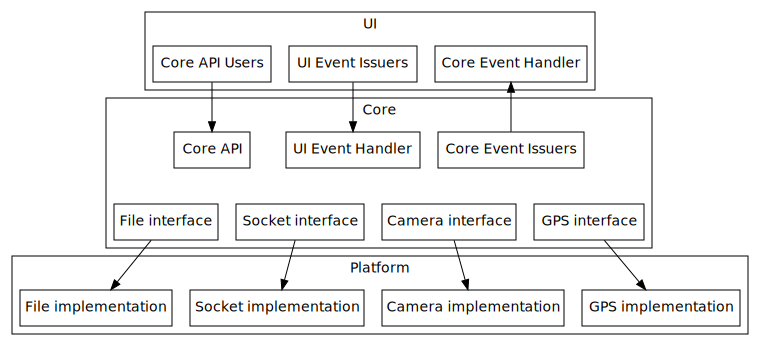
\includegraphics[scale=0.4]{08_2015_fig1}
\end{figure}

Приложение состоит из 3 частей:

\begin{itemize}
  \item UI "--- реализация UI, платформо"=зависимый код.
  \item Core "--- ядро/движок, платформо"=независимый код.
  \item Platform "--- реализация поддержки файловой системы, сети и устройств, платформо"=зависимый код.
\end{itemize}

Стрелки на схеме означают:

\begin{itemize}
  \item CoreAPIUsers $\rightarrow{}$ CoreAPI "--- Команды от UI к Core, например <<Перейти на такой"=то URL в таком"=то табе>>.
  \item UIEventIssuers $\rightarrow{}$ UIEventHandler "--- События в UI, которые должны быть обработаны Core, например клик мыши.
  \item CoreEventIssuers $\rightarrow{}$ CoreEventHandler "--- События в Core, которые должны быть обработаны в UI, например перерисовка области экрана.
  \item Some interface $\rightarrow{}$ Some implementation "--- вызовы кода, реализующие <<платформенный интерфейс>>, то есть отвечающего за поддержку файловой системы, сети и устройств на данной платформе.
\end{itemize}

Таким образом, для того, чтобы добавить поддержку какой"=либо платформы, надо:

\begin{itemize}
  \item Решить, какие возможности браузера и устройства хочется поддерживать на этой платформе.
  \item Разработать реализацию UI и платформенных интерфейсов, с учётом выбранных возможностей.
\end{itemize}

То есть, если какая"=то возможность браузера (например, поддержка GPS) не будет активирована на данной платформе "--- не надо и реализовывать платформенный интерфейс GPS"=устройства. Подробнее включение/отключение возможностей программы будет описано ниже.

\subsection*{Как решать проблемы}


\begin{figure}[h!]
  \centering
  \begin{tabular}{ p{4.3cm} p{6.2cm} } \hline
    \textbf{Проблема}                                          & \textbf{Решение}                                                                                      \\ \hline
    Разные скорости CPU и объёмы памяти                 & Включение/отключение возможностей на стадии компиляции                                         \\
    Разные размеры экранов и их количество              & Задание размера экрана/окна при инициализации/изменении                                        \\
    Разные устройства управления                        & Поддержка в UI layer, возможно частично в Platform layer                                       \\
    Разные дополнительные устройства (камера, GPS) & Поддержка в Platform layer, обязательный \verb@#ifdef SOME_DEVICE_SUPPORT@                          \\
    Разные компиляторы, в том числе и капризные (ADS)   & Ответственное использование С++ (namespaces, templates, exceptions, RTTI, global vars, static) \\
    Особые методы запуска приложений (BREW, P2K)        & Реализация UI как библиотеки                                                                   \\
    Разные API у разных операционных систем             & Поддержка в Platform layer                                                                     \\ \hline
  \end{tabular}
\end{figure}

Выше были упомянуты некоторые проблемы, присущие кроссплатформенной разработке. Приведенная таблица кратко описывает, как их решать.

\subsection*{Включение/отключение возможностей на стадии компиляции}

Некоторые платформы, например feature phones имеют не очень"=то много памяти, как для хранения кода приложения, так и для его работы. Отключение некоторого функционала приложения на стадии компиляции помогает уменьшить размер кода этого приложения, расход памяти, а также ускоряет его работу.

Также, чем менее мощны устройства определённой платформы "--- тем, как правило, меньший спектр встроенных устройств (камера, GPS, etc) они поддерживают. Код для неподдерживаемых встроенных устройств на данной платформе также следует исключать из компиляции.

Для того, чтобы реализовать отключаемую поддержку определённого функционала или устройств на стадии компиляции для определённой платформы, используется простой способ:

\begin{enumerate}
  \item Обрамить код поддержки отключаемого функционала или \linebreak устройства в \#ifdef SOME\_FEATURE\_SUPPORT.
  \item Описывать (\#define) или сбрасывать (\#undef) соответствующий макрос в глобальном заголовочном файле для соответствующей платформы.
\end{enumerate}

Ниже приведён фрагмент кода на C++, который иллюстрирует описанный способ:

\begin{verbatim}
    #define FEATURE_1_SUPPORT
    #undef  FEATURE_2_SUPPORT
        ...
        // Код feature 1 будет скомпилирован,
        // потому что решено поддерживать
        // feature 1 на этой платформе.
    #ifdef FEATURE_1_SUPPORT
        m_component_loader->LoadFeature1Data();
    #endif
        ...
        // Код feature 2 не будет скомпилирован,
        // потому что решено не поддерживать
        // feature 2 на этой платформе.
        // Это уменьшит размер исполняемого кода,
        // потребление памяти во время исполнения
        // и увеличит его скорость.
    #ifdef FEATURE_2_SUPPORT
        m_component_loader->LoadFeature2Data();
    #endif
        ...\end{verbatim}
\subsection*{Как ещё уменьшить размер кода}

Существуют также и другие способы уменьшить размер кода:

\begin{itemize}
  \item Использовать код повторно, удалять более неиспользуемый код
  \item Уменьшить размер временных буферов и/или их время жизни (совет для runtime)
  \item Больше использовать библиотеки платформы, не дублировать их функционал в коде приложения
  \item Урезать используемые third"=party библиотеки, всё"=таки включённые в приложение; таким же образом (\#undef FEATURE), как урезается основной код
  \item Избегать зависимостей от слабых мест компилятора, (пример: раздувание template"=кода)
  \item Кросс"=компилировать лучшим компилятором
  \item Компилировать в более компактный набор инструкций процессора (пример: Thumb для ARM)
  \item Сжимать код, в ROM или RAM
  \item Использовать плагины/оверлеи
  \item Исполнять части кода в другом месте (пример: Opera Mini)
\end{itemize}

\subsection*{Пример платформенного интерфейса}

Ниже приведён пример платформенного интерфейса для сокетa TCP. Реализовав этот платформенный интерфейс, разработчик \linebreak обеспечит работу TCP"=соединений на данной платформе. Для Unix"=подобной платформы реализация может использовать BSD sockets, для Windows "--- WinSock, для Telium OS "--- LinkLayer и т.~д.

\begin{verbatim}
    // Будет реализовано в платформенном коде.
    class TCPSocket
    {
        static TCPSocket* New();
        Status SetListener(TCPSocketListener* listener) = 0;

        Status Connect(const char* host, unsigned short 
port) = 0;
        Status Disconnect() = 0;
        Status Send(const char* data, size_t length, size_t& 
accepted_length) = 0;
        Status Recv(char* data, size_t length, size_t& 
received_length) = 0;
    };

    // Будет реализовано в коде ядра.
    class TCPSocketListener
    {
        Status OnConnected() = 0;
        Status OnDisconnected() = 0;
        Status OnDataSent(size_t length) = 0;
        Status OnDataAvailable(size_t length) = 0;
        Status OnError(Error code) = 0;
    };
\end{verbatim}
\end{document}
